\section{Aggregation}
For aircraft wing design, currently, there is a trend to employ higher-fidelity (more expensive) and multidisciplinary numerical simulations, such as the coupling of CFD code and CSD code. In addition, optimization problems become more and more complex, with many design variables, tightly coupled objectives, and a large number of constraints. Handling large-scale constraints presents a challenge for wing structural and aero-structural design, since the refined finite element model with multiple freedoms incurs millions of structural failure constraints. \cite{zha}\\
In our optimization problem we are also interested to minimize the structural mass subject to constraint on structural failure, in particular we are interested in failure based on yield stress. In the design checking the failure criteria in the optimization process is desirable, because allow to verify that the optimized structure is suitable for the prescribed load conditions.\\
The primary issue with including failure constraints directly in the structural optimization problem is the resulting size of the optimization problem. Conceptually, for a continuum structure, failure constraints need to be enforced throughout the material domain, leading to an infinite number of constraints. More practically, failure constraints may be enforced element-wise in the finite element model. For detailed, high-fidelity structural models, this can lead to an optimization problem with many thousands or millions of failure constraints. These constraints are costly to enforce because they can only be checked by completing the structural analysis.\cite{lambe}\\
Aggregation methods allow to manage an huge number of constraints, in fact that methods lump a large number of constraint into one global constraint, so the computational cost of the multidisciplinary optimization drastically decrease. These methods consist in the use of an aggregation function, which transform a set of local function values into a scalar function. This scalar function converge in the limit to the maximum local function value:
\begin{equation*}
\lim_{P\to\infty} G(\mathbf{f},P)=\max(f_1,f_2,...,f_N)
\end{equation*}
where $\mathbf{f}$ = $(f_1,f_2,...,f_N)^T$ is a vector in which the entries are the local function values, $G$ is the scalar aggregation function and $P$ is the draw-down factor that manage the aggregation.\\
There are different aggregation function, some of them approximate the maximum of the local function from above, and other from belove. So depending on this characteristic behavior aggregation function forms an upper or lower bound to the maximum local function value.\\
Related to our problem aggregation function became necessary for the stress failure constraints, in fact when the structural model is detailed, so the number of elements became huge, we need to check the stress criteria on each single element; this entails that need one constraint for each element in the optimization process, with the result that the computational cost became prohibitive, and openMDAO find problem in the setup phase to creates this huge number of constraint, and sometimes it can crash in this phase.Additionally using a gradient-based optimizer the aggregation fucntion can avoid the problem of the not differentiable maximum function, increasing the curvature of the function in the region where there is this problem modifying the draw-down factor. That's one of the reason because we implemented a new component in the optimization process, the aggregation component, so the XDSM of the optimization process is modified as follow:
\begin{figure}[H]
	\centering
	\includegraphics[width = 0.8\textwidth]{./Immagini/3_1.png}
	\caption{XDSM after constraints aggregation}
	\label{fig:3_1}
\end{figure}
As we can see after the implementation of the aggregation component a new box function have been added, the box function 11. So after the extraction of the Von Mises stresses vector by the structural component the aggregation component take this vector as input and give as output the scalar $G$. Now the constraint function is connected to$G$ and to $\sigma_{yeild}$, so the constraint will be determinate using these variables.
\subsection{Aggregation Method}
Let's see how the aggregation implementation modifies the approach of the optimization design problem, and in particular referred to our problem. \\
Suppose the original problem is to optimize the mass of a structure under the failure criteria constraint, the problem in this case can be written as:
\begin{align*}
&minimize \qquad \quad m\\
&subject\ to \qquad  \sigma_{VM_i}< \sigma_{Yield}\qquad \forall \ i=1,2,...,N
\end{align*}
where $m$ is the mass of the structure, $\mathbf{\sigma_{VM}} =[\sigma_{VM_1},\sigma_{VM_2},...,\sigma_{VM_N}]$ is the vector containing the Von Mises stresses of each finite element used for the structural analysis, $\sigma_{Yield}$ is the yield stress and $N$ is the number of the finite elements.\\
Let's see how the problem is modified using the maximum constraint approach, the simplest aggregation method. Using this method we have that the most violated constraint is selected, while the rest are ignored. \\In this case the problem can be written as:
\begin{align*}
&minimize \qquad \quad m\\
&subject\ to \qquad  \max (\sigma_{VM_i})< \sigma_{Yield}\qquad  \ i=1,2,...,N
\end{align*}
However, because the constraints is not smooth it's not possible to use a gradient-based algorithms in the optimization process, and the search direction is determined by considering only the Lagrange multipliers of the most violated constraint, usually leading to the violation of another constraint in the next iteration.\\
Using an constraint aggregation function the optimization is subject to the value of the aggregation function $G$, so the problem can be written as:
\begin{align*}
&minimize \qquad \quad m\\
&subject\ to \qquad  G < 0
\end{align*}
where $G$ is a scalar, given from the aggregation function and it's representative of the maximum value of the Von Mises stresses vector. $G$ depends, as we said, also to the aggregation function choose, so in the next paragraph we will introduce the most common aggregation function, and theirs properties.
\section{Aggregation Functions}
In literature several aggregation function have been used. The choice of the function depends of the nature of the problem, of the size of the problem and of the properties required to perform the analysis. For the failure criteria, where the constraint impose the stresses lower than yield stress, the natural choice for these constraint aggregates is a maximum- or minimum-value function. But the problem it's that this kind of functions are not differentiable, so cannot be used efficiently in gradient-based optimization. Another choice can be the \textbf{p-mean} and \textbf{p-norm} function, or the \textbf{Kreisselmeier-Steinhauser KS} function, kind of smooth estimator. These estimators do not precisely reproduce the true feasible design space provided by the original constraints, so the final design determined by the optimizer will be different depending on the aggregation scheme. \cite{lambe} 
\subsection{Function}
First, we briefly discuss aggregation function used in the literature.\\
About the nomenclature we use $G$ to indicate the aggregation function, the superscript $_L$ and $_U$ to denote respectively an lower- or upper-bounded aggregation function, and $P$ to indicate the draw-down factor.\\
The first two aggregation function that we analize is the \textbf{p-norm} and the \textbf{p-mean} function. This kind of aggregation function can be use when the local function value $\mathbf{f}$ are non-negative, as in our case where $\mathbf{f}$ is the Von Mises stresses vector, so for definition we have that all the component of the vector, the Von Mises stress of each finite element, is positive.
\subsubsection{P-norm}
\begin{equation}
G_{PN}^U=\left(\sum_{i=1}^{N}f_i\right)^{1/P}
\end{equation}
\subsubsection{P-mean}
\begin{equation}
G_{PM}^L=\left(\frac{1}{N}\sum_{i=1}^{N}f_i^P\right)^{1/P}
\end{equation}
The difference between these two aggregation functions is that the P-norm is an upper bound, and the P-mean is a lower bound to the maximum local function value:
\begin{equation*}
G_{PM}^L \le \max(f_1,f_2,...,f_N)\le G_{PN}^U
\end{equation*}
For this propriety it's important to note, in the implementation in an optimization process, that the p-norm function is conservative, backwards the p-mean is not conservative.
\subsubsection{Kreisselmeier-Steinhsauser function}
The Kreisselmeier-Steinhsauser aggregation function have been presented for the first time by G. Kreisselmeier and R. Steinhsauser \cite{krei}.The function constains a “draw-down” factor or aggregation parameter, $P$, which is analogous to the penalty factor in penalty methods used to perform constrained optimization \cite{poon2}.\\
This function have been used first to aggregate multiple objectives and constraints into single functions, but in the time became popular to be used in the direct constrained optimization problem. This function has few important proprieties, about we will discuss after, but ne of the more important property is the following: "The function produces an envelope surface that is $C1$ continuous and represents a conservative estimate of the maximum among the set of functions" \cite{nasa}.\\
The KS function can be used also to aggregate only the constraints into a single continuous function, in that way is defined as:
\begin{equation}
G_{KS}^U=\frac{1}{P}\ln\left(\sum_{i=1}^{N}e^{Pf_i}\right)
\end{equation}
This function, as the superscript denote, is an upper bounded function, for each $P>0$, so it overestimates the maximum local function value. Let's see the properties of this function:
\begin{align*}
G_{KS}(x,P)\ge\max(f_i(x))                     &\qquad for \qquad P>0\\
\lim_{P\to\infty}G_{KS}(x,P)=\max(f_i(x))& \qquad for \qquad j=1,2,...,N\\
G_{KS}(x,P_1)\ge G_{KS}(x,P_2)             &\qquad for\qquad  P_1>P_2>0\\
G_{KS}(x,P) \qquad\qquad                     &\qquad is\ convex,\  if\  and\  only\  all\  constraint\  are\  convex
\end{align*}
These properties is really important for the KS function to be considered an valid aggregation function. The first three properties indicate, as we said, that the KS function is upper-bounded, it overestimates the maximum of the constraint defined as $G_i\le0$, a positive value returned indicate that a constraint is violated or close to being violated. The conservative nature is determined from the aggregation parameter $P$, id $P$ increases the aggregation function value became more closer to the maximum value. The effect of the aggregation parameter will be investigate in the next paragraph, but in Fig. \ref{fig:3_2} we can see that effect from the investigation done by J. R. R. A. Martins, for a two constraints problem, $g_1$ and $g_2$: \cite{poon2}:
\begin{figure}[H]
	\centering
	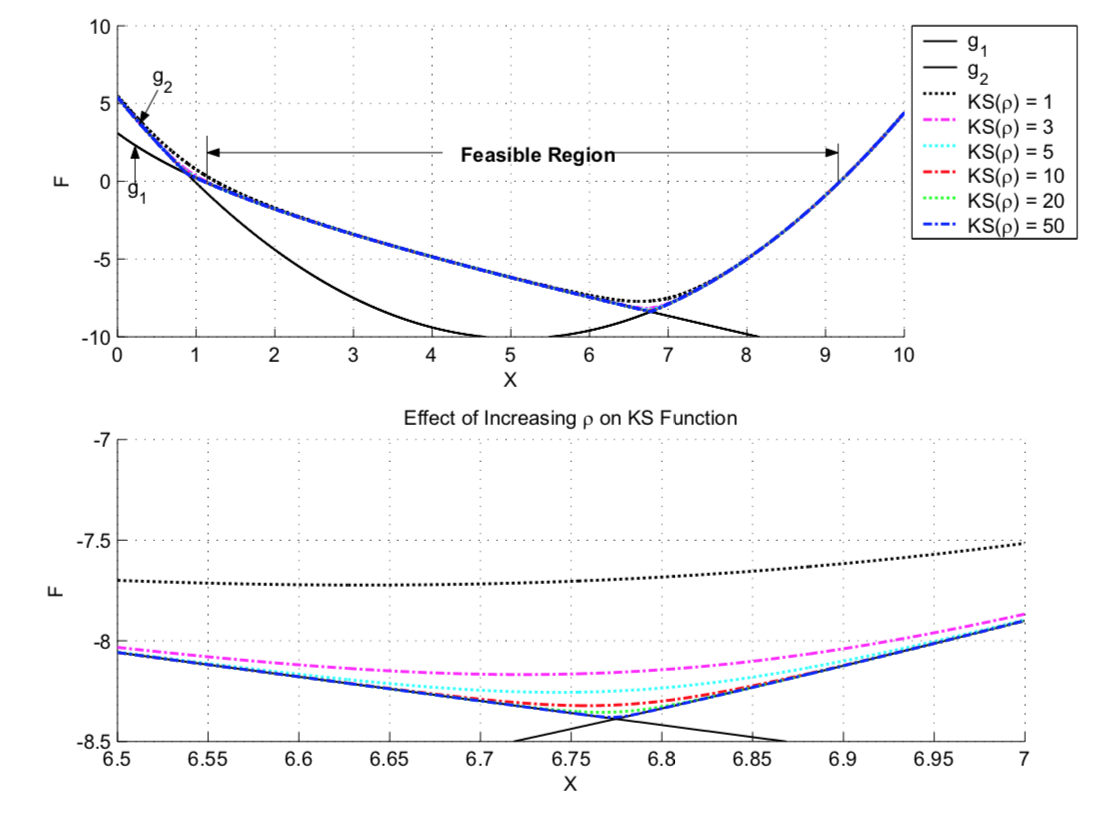
\includegraphics[width = 0.8\textwidth]{./Immagini/3_2.png}
	\caption{Effects of the aggregation parameter $P$ on the KS function}
	\label{fig:3_2}
\end{figure}
An alternative formulation can be used, to avoid numerical difficulties caused by numerical overflow, the KS function can be written as:
\begin{equation}
G_{KS}^U=f_{max}+\frac{1}{P}\ln\bigl[\sum_{i=1}^{N}e^{P(f_i-f_{max})}\bigr]
\end{equation}
where $f_{max}$ is the max value of the local function.\\
The maximum difference between the maximum value of the local function and the value of the aggregation function is determinate by $P$, and it's value its:
\begin{equation}
\frac{1}{P}\ln\left(Ne^{Pf_{ma}}\right)-f_{max}=\frac{1}{P}ln(N)
\end{equation}
that's mean:
\begin{equation}
f_{max}<G_{KS}<f_{max}+\frac{1}{P}ln(N)
\end{equation}
From this property can be obtained an alternative formulation of the KS function, a lower bounded KS function. To obtain it we need to subtract the maximum difference between the maximum of the local function to the KS upper bounded function, obtaining :
\begin{equation}
G_{KS}^L=G_{KS}^U-\frac{1}{P}ln(N)=\frac{1}{P}ln\left(\frac{1}{N}\sum_{i=1}^{N}e^{Pf_i}\right)
\end{equation}
that became the following using the alternative formulation:
\begin{equation}
G_{KS}^L=f_{max}+\frac{1}{P}\ln\bigl[\sum_{i=1}^{N}e^{P(f_i-f_{max})}\bigr]-\frac{1}{P}ln(N)
\end{equation}
\subsection{Effects of the Aggregation Parameter $P$}
The aggregation parameter or draw-down factor $P$ has several effects on the aggregation function. Choose it correctly is really important to have low relative error of aggregation function relatively at the real maximum of the local function, and also a low computational cost. The right choice of the aggregation parameter depends as first of the problem size, but also from the dispersion of the value of the local function and their absolute value. In addiction is important to choose the draw-down factor to smooth the aggregation function in the region where the constraints intersect, to be possible to compute the derivatives.\\
As first we can see in Fig. \ref{fig:3_3} how the size of the problem influence the relative error for a given draw-down factor. We use the aggregation function to aggregate the Von Mises stresses vector, so the value of the aggregation function is representative of the maximum stress for the finite elements of the structure. In this case we choose a Kreisselmeier-Steinhsauser function lower bounded, we set the draw-down factor as 50, then we compute the relative error as:
\begin{equation*}
\epsilon = \left| \frac{G_{KS}^L-f_{max}}{f_{max}} \right|
\end{equation*}
Than we compute the relative error for different size of the stresses vector. Locking the draw-down factor we can see how the relative error grow with the size of the problem, or analogously with the number of the constraints that we want to aggregate.
\begin{figure}[H]
	\centering
	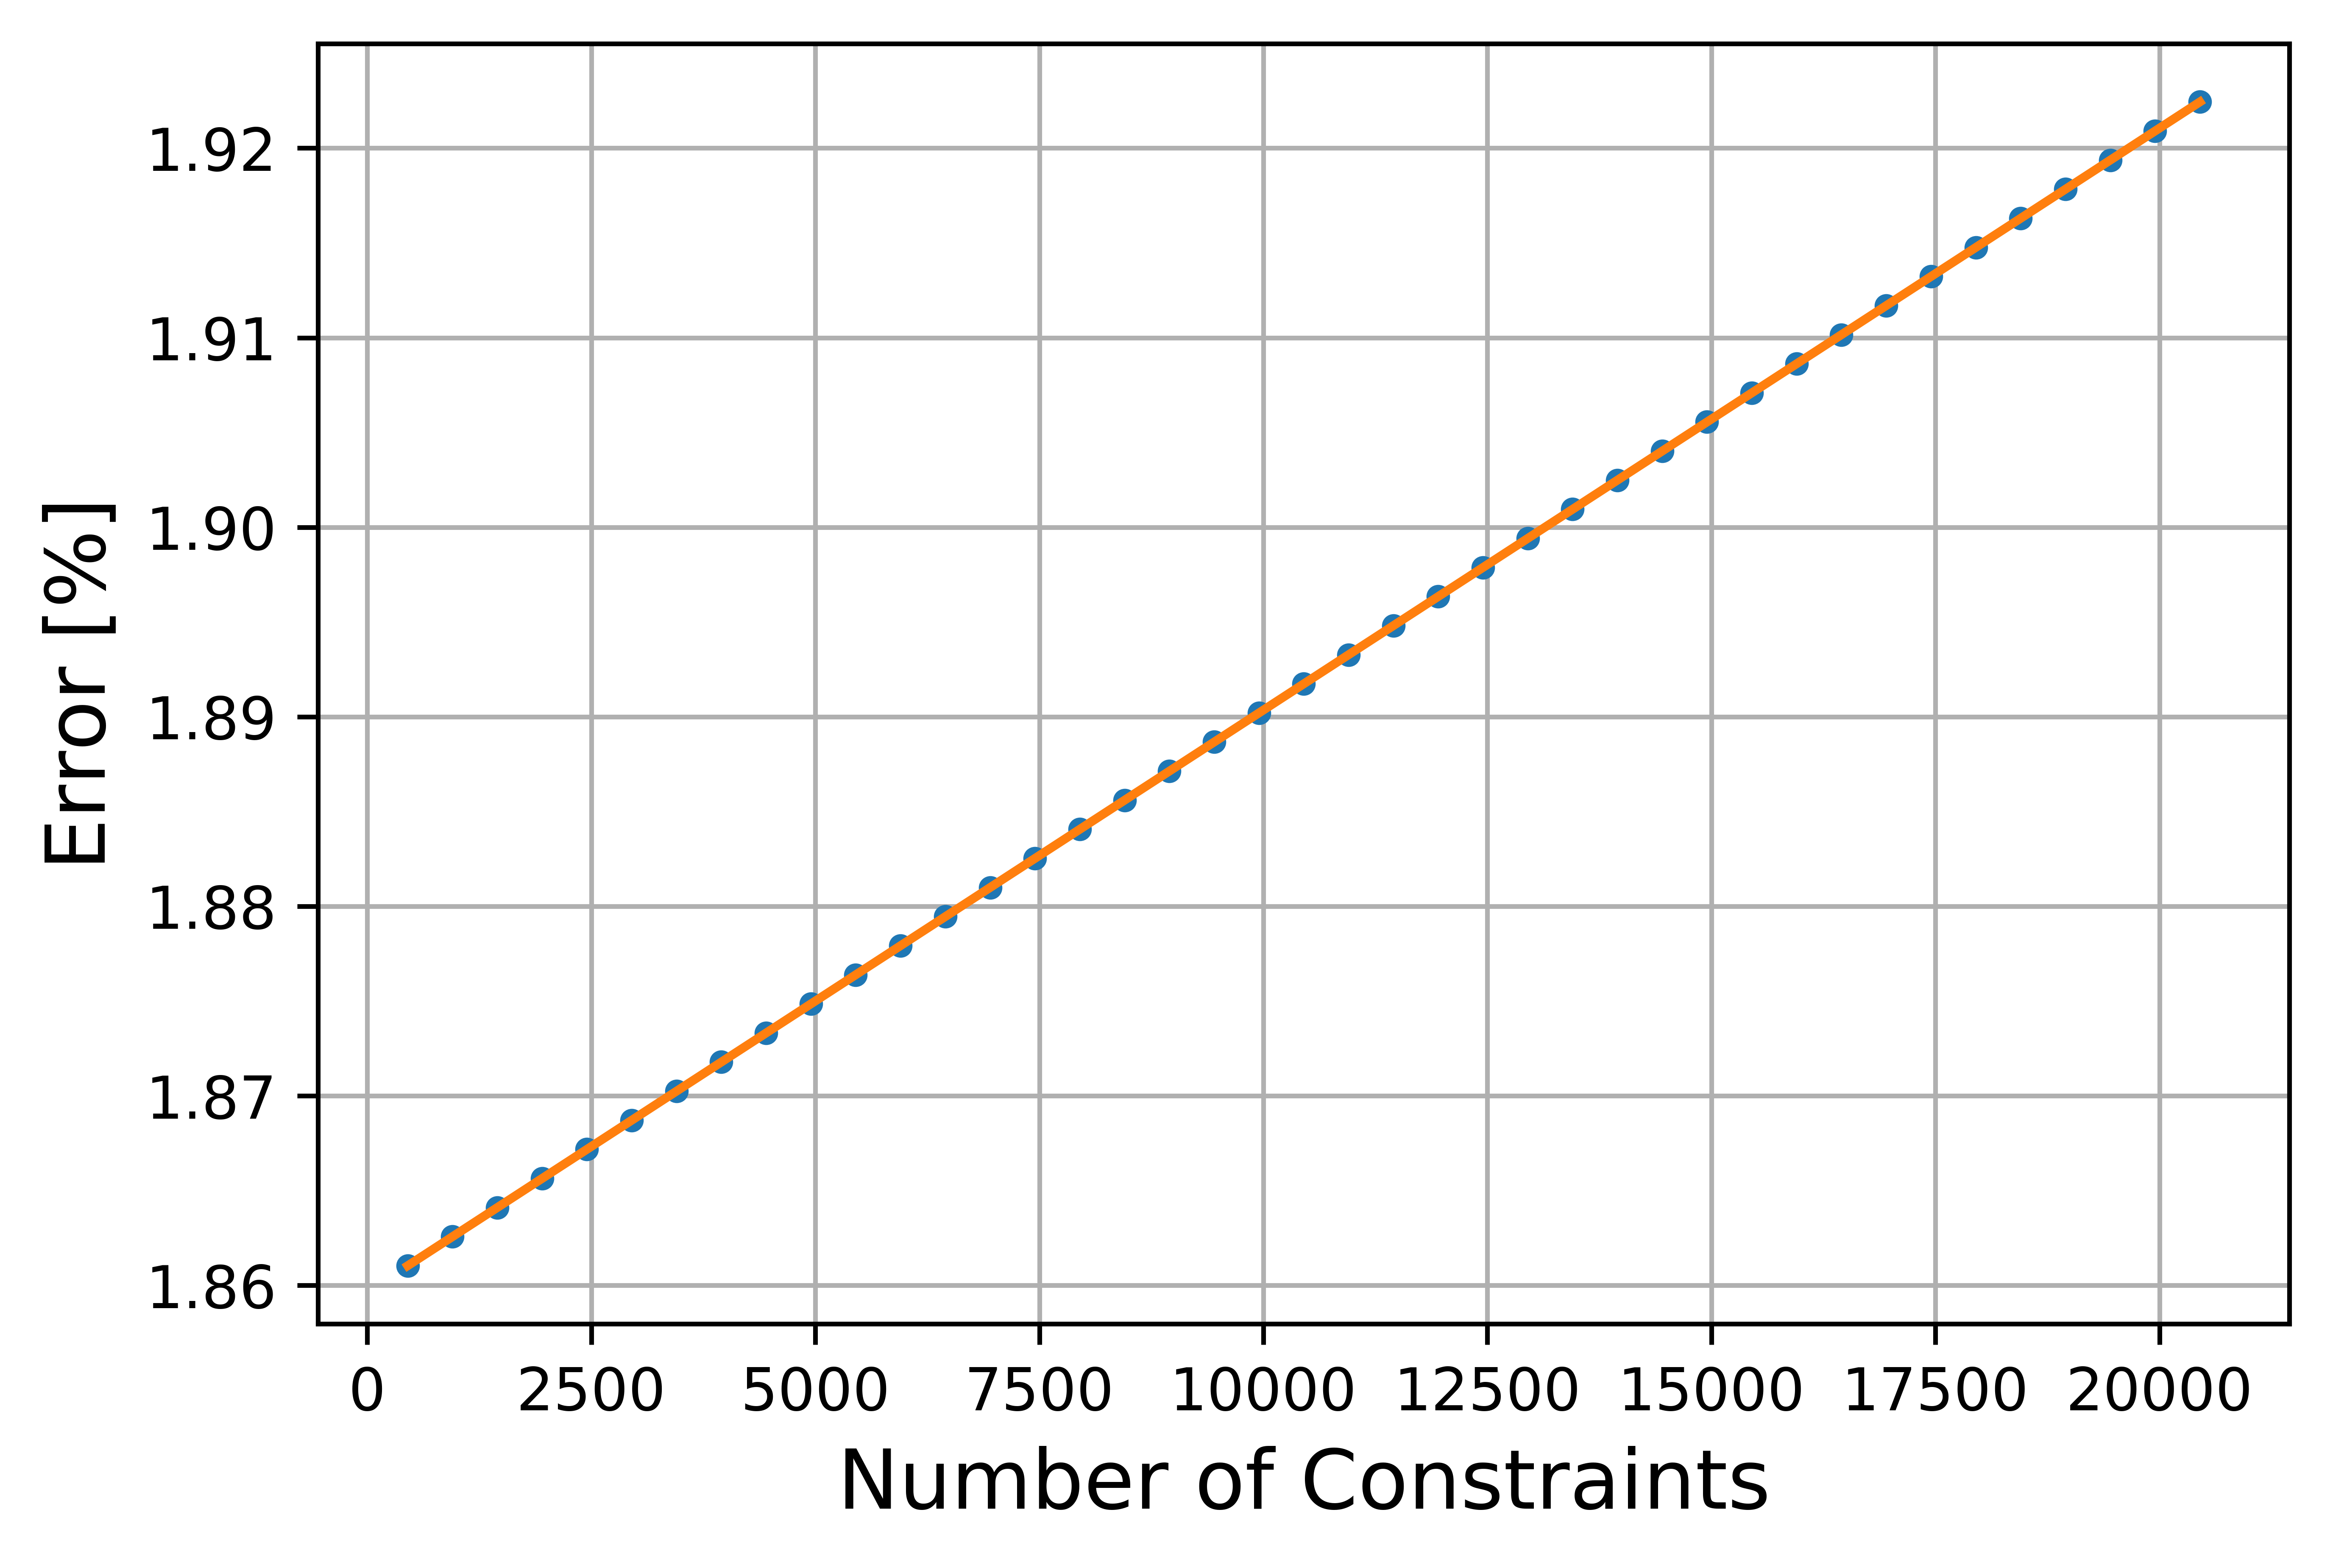
\includegraphics[width = 0.8\textwidth]{./Immagini/3_3.png}
	\caption{Effects of the number of constraint on the relative error of the aggregation function}
	\label{fig:3_3}
\end{figure}
The choice of aggregation parameter is also constrained to the aggregation function and to the maximum relative error. In Fig. \ref{fig:3_4} there are showed how the relative error changes with the aggregation parameter for the different aggregation function implemented in the code. To obtain this graph we take one Von Mises stresses vector as example, and we determinate the aggregation function value for different value of the aggregation parameter, then we compare the aggregation function value with the maximum of the stress vector obtained with the maximum-value function:
\begin{figure}[H]
	\centering
	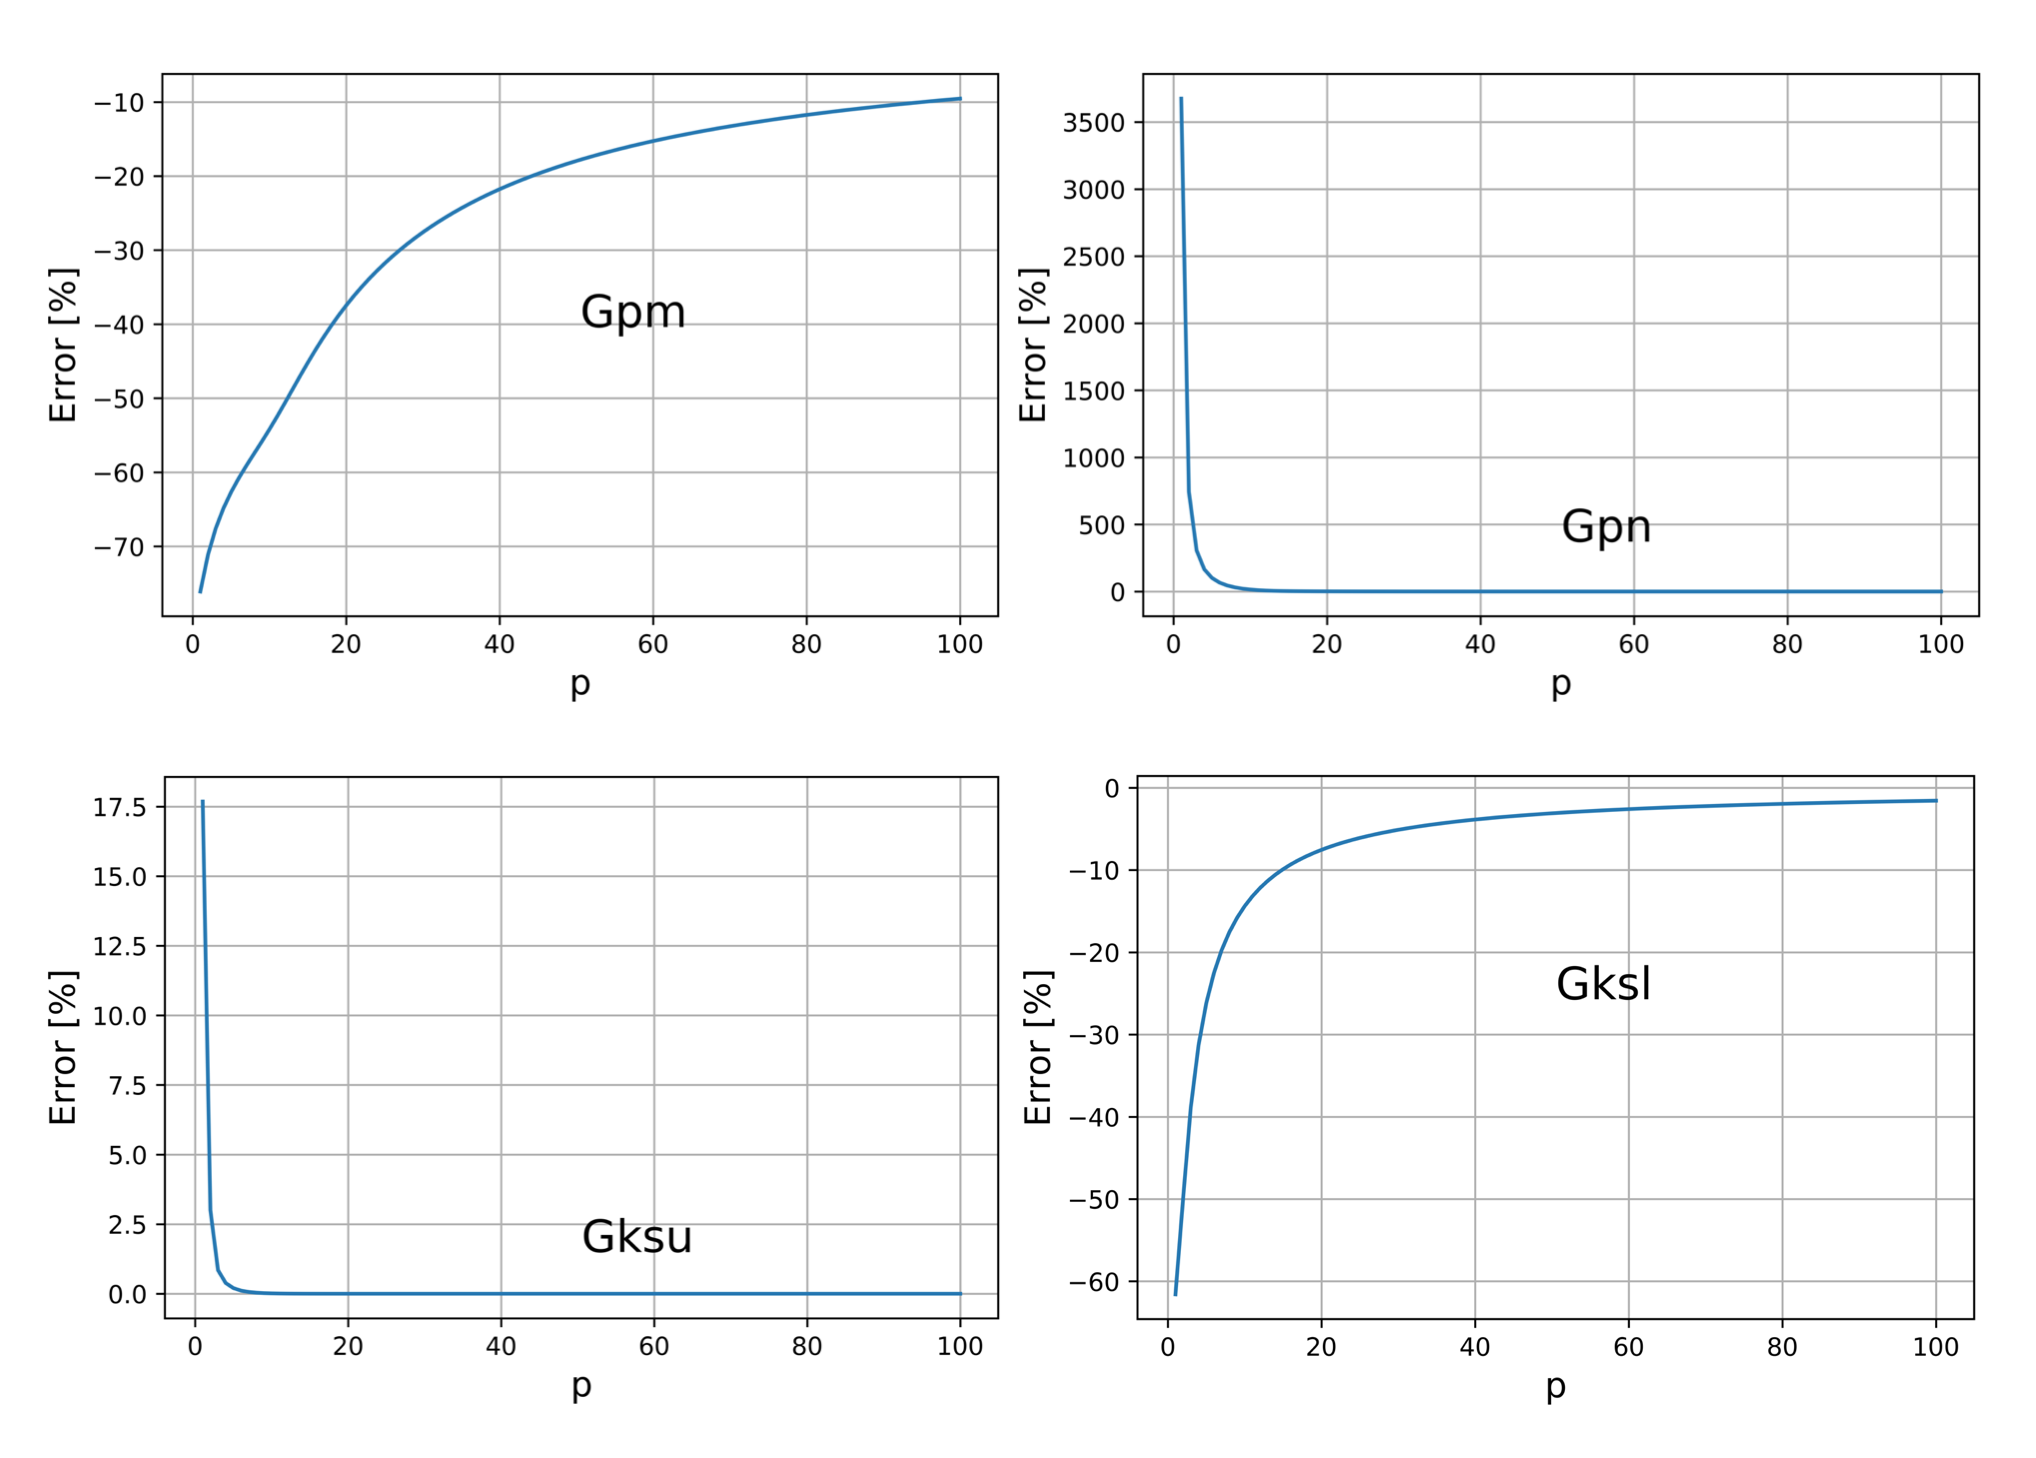
\includegraphics[width = 0.7\textwidth]{./Immagini/3_4.png}
	\caption{Effects of the aggregation parameter $P$ on the relative error}
	\label{fig:3_4}
\end{figure}
From these graphics we can saw the difference between a lower bounded function ($G_{KS}^L$ and $G_{PM}^L$) or an upper bounded function ($G_{KS}^U$ and $G_{PN}^U$), in fact as we can see in the first case the relative error converge to 0 from the bottom, and in the second case from the top. As we can see, as definition, for $p\to\infty$ the relative error go to 0, and that error depends from the aggregation function, the relative error is acceptable for $P\approx 50$ for the upper bounded function, while for the lower bounded the error is still not acceptable. "$P = 50$ is usually a reasonable value that has a maximum relative error of $\approx$ 0.03 for two constraints, and is often used"\cite{stu}.\\
In Fig. \ref{fig:3_5} it's showed an zoom-out to see also the upper-bounded function reach the convergence.
\begin{figure}[H]
	\centering
	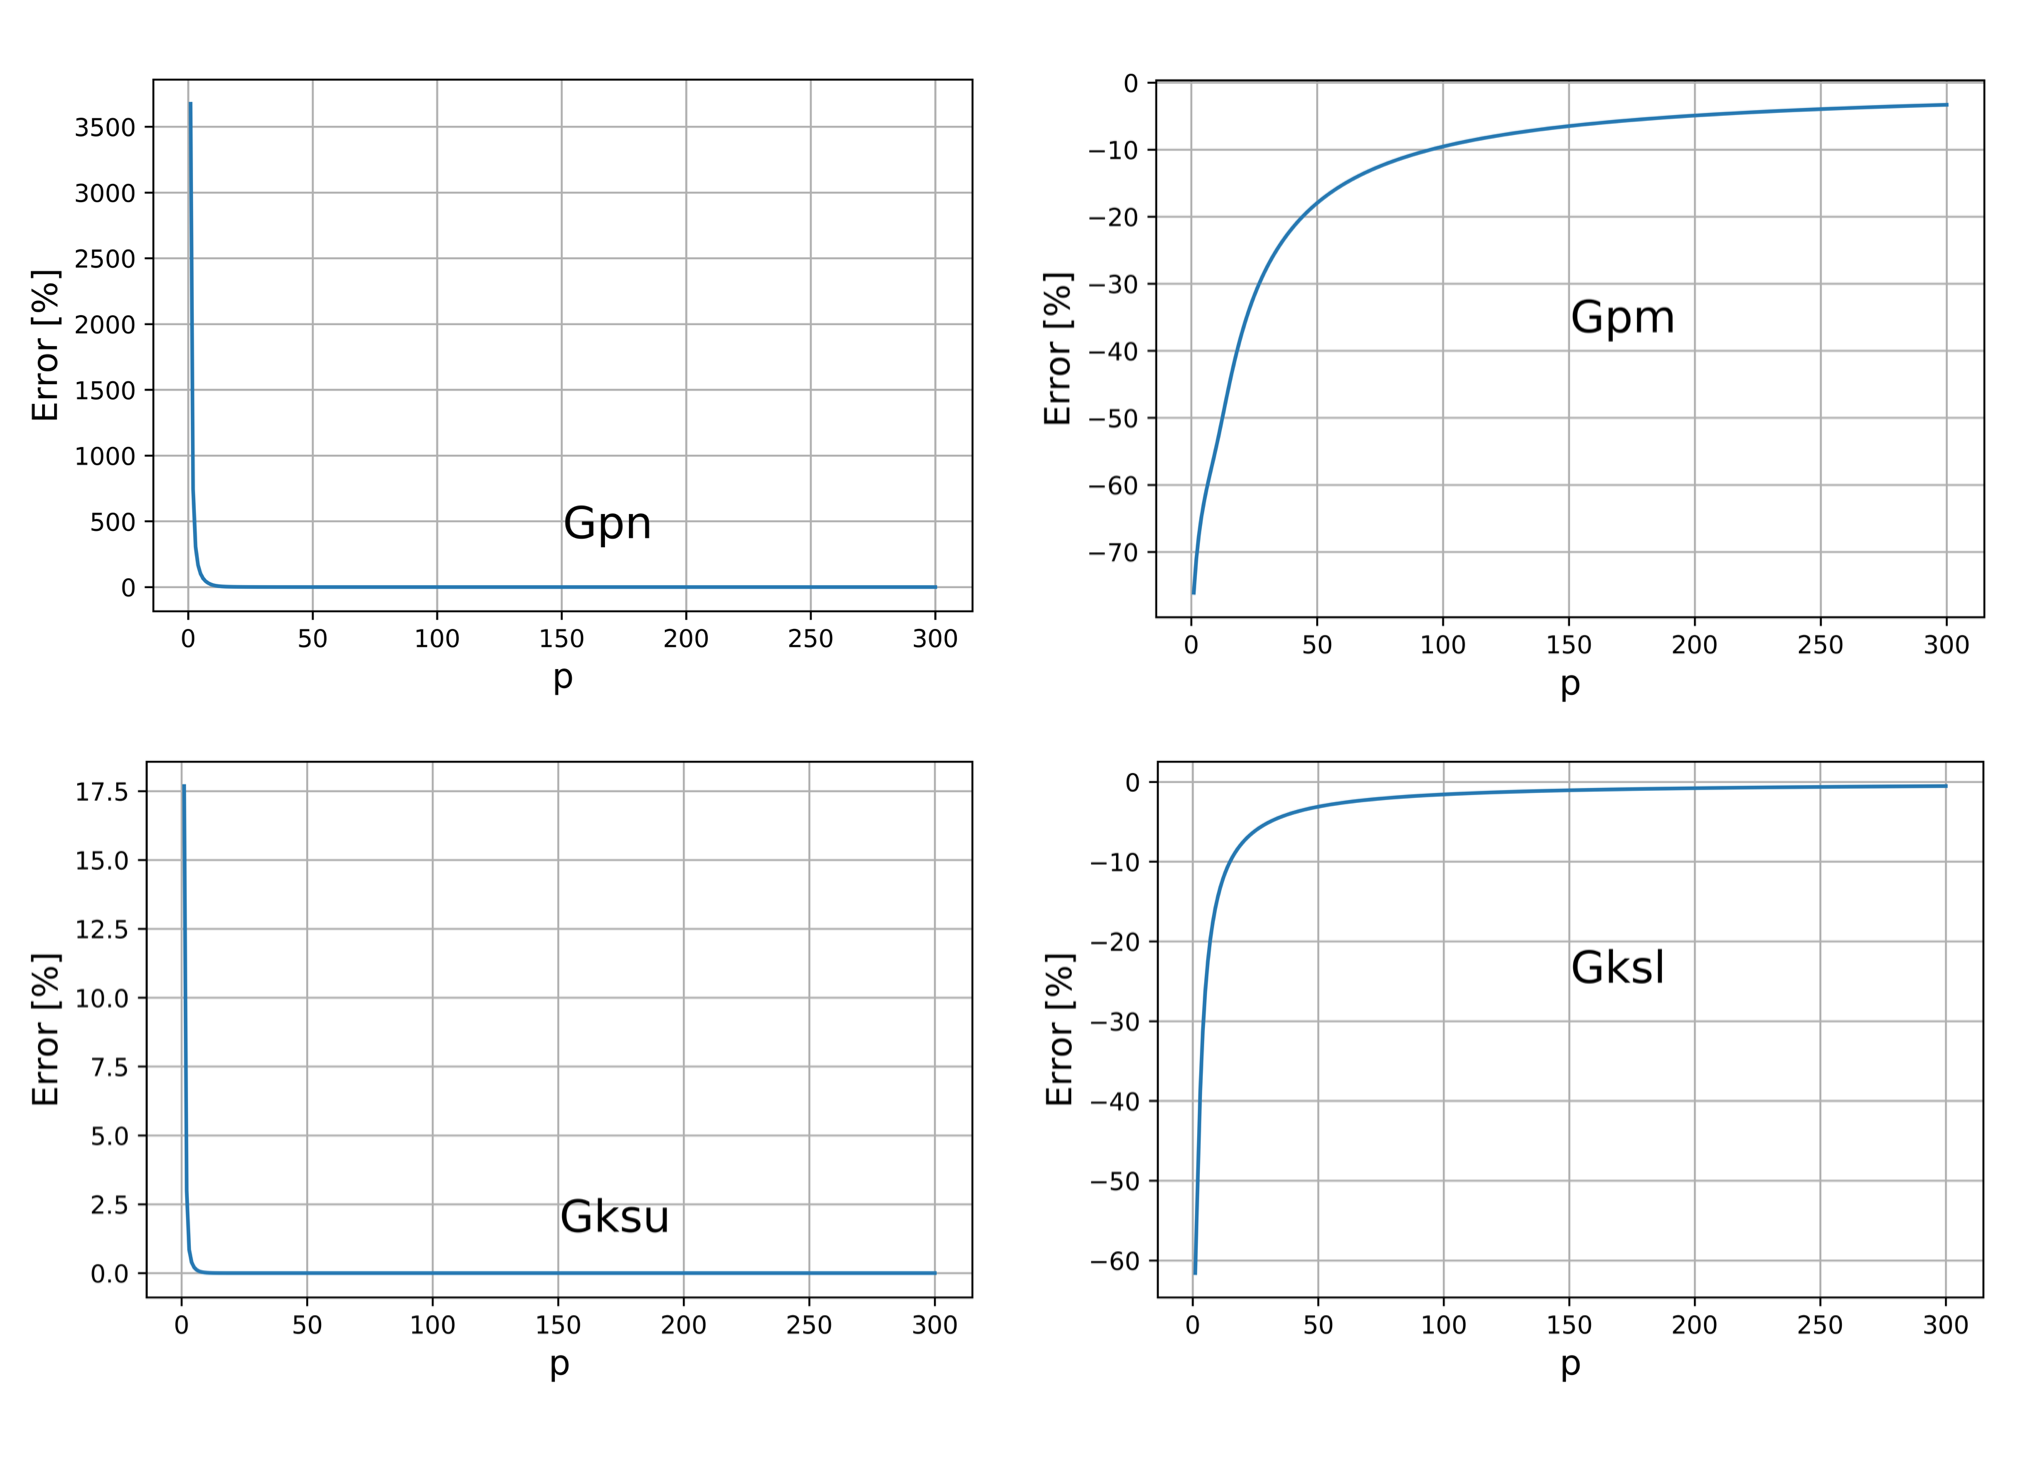
\includegraphics[width = 0.7\textwidth]{./Immagini/3_5.png}
	\caption{Zoom-out of effects of the aggregation parameter $P$ on the relative error}
	\label{fig:3_5}
\end{figure}
\section{Aggregation Component}
To implement the constraint aggregation in the optimization code needs a component that take as input the Von Mises stresses vector and give as output the value of the aggregation function. To be implemented in our script the component should be written in the openMDAO structure. In Fig. \ref{fig:3_6} is represented the flow chart of the component.
\begin{figure}[H]
	\centering
	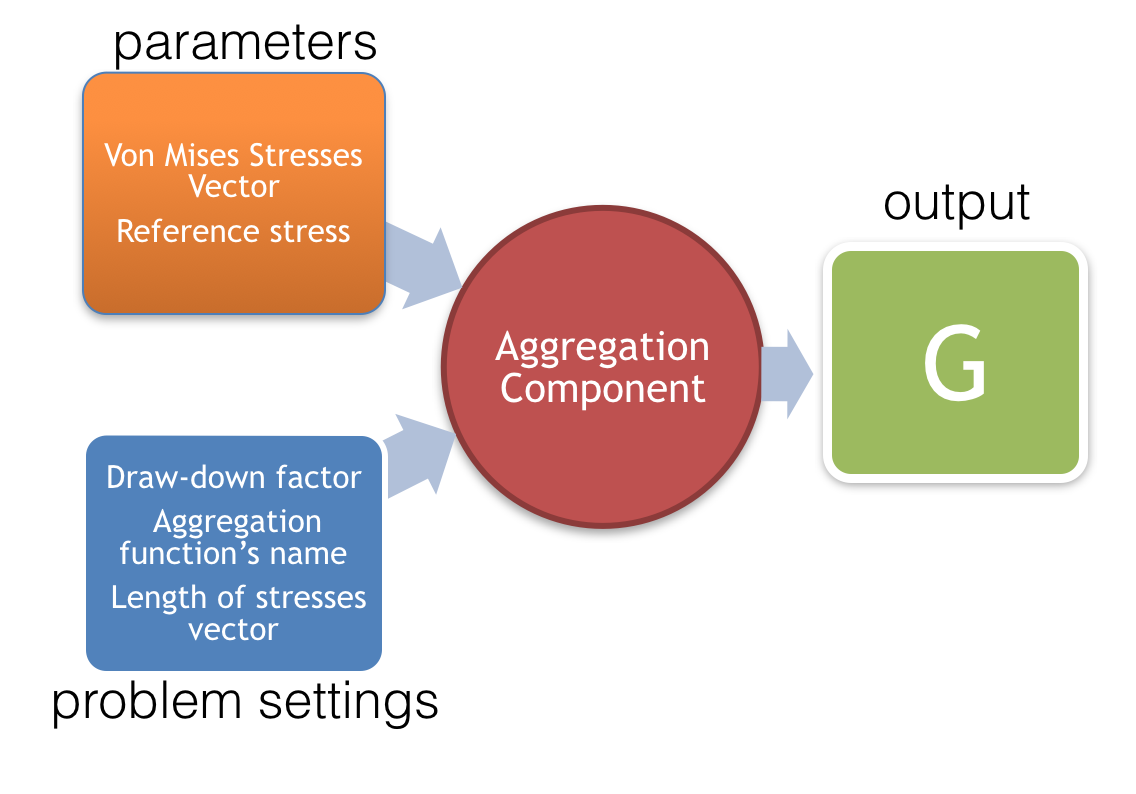
\includegraphics[width = 0.8\textwidth]{./Immagini/3_6.png}
	\caption{Flow chart of the aggregation component}
	\label{fig:3_6}
\end{figure}
The aggregation component takes as input parameters the Von Mises stresses vector $\mathbf{\sigma_{VM}}$ and the reference stress $\sigma_0$ used for the nondimensionalization, connected to the relative variables of the main code between the command \textit{promotes=[*]}; the settings of the aggregation are declared in the main script and are input for the component, there are the value choose for the draw-down factor, the aggregation function selected and the dimension of the vector. Than the component compute the aggregation function and give as output it's value, joined to the constraints functions to be used during the optimization process.\\
In Fig. \ref{fig:3_7} it's showed how the component is made, in the openMDAO structure and the links between the variables:
\begin{figure}[H]
	\centering
	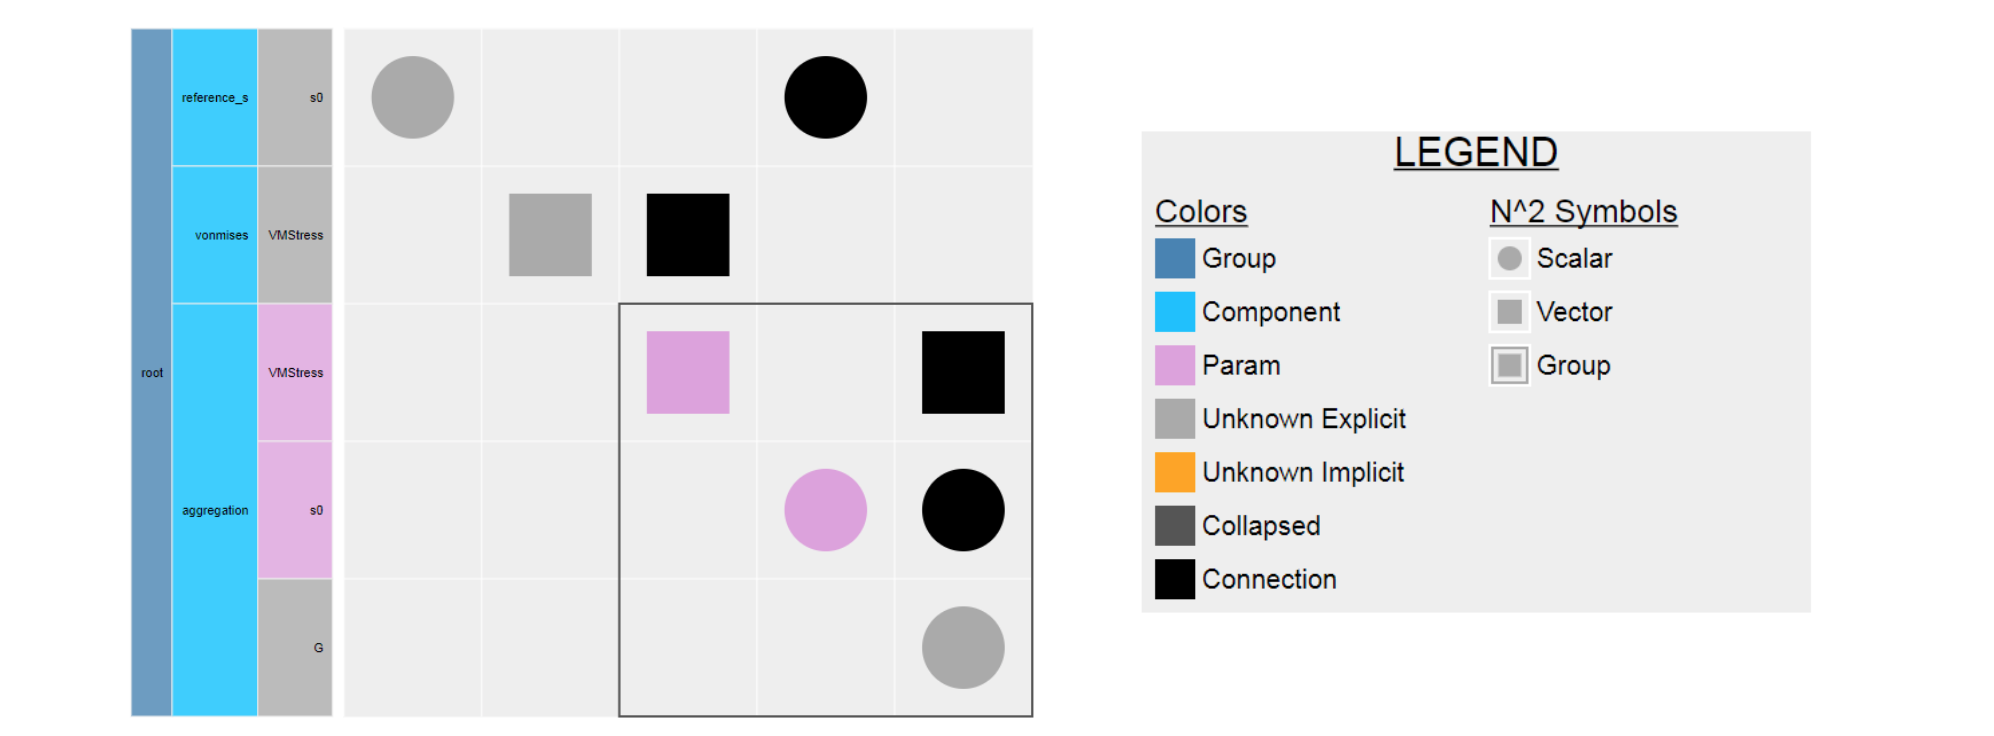
\includegraphics[width = 1\textwidth]{./Immagini/3_7.png}
	\caption{openMDAO structure of the aggregation component}
	\label{fig:3_7}
\end{figure}
